\pdfoptionpdfminorversion=7
\documentclass{beamer}

\mode<presentation>
{
  \usetheme{Madrid}       % or try default, Darmstadt, Warsaw, ...
  \usecolortheme{default} % or try albatross, beaver, crane, ...
  \usefonttheme{serif}    % or try default, structurebold, ...
  \setbeamertemplate{navigation symbols}{}
  \setbeamertemplate{caption}[numbered]
}

\usepackage{amsmath}
\usepackage[utf8x]{inputenc}
\usepackage{listings}
\usepackage{graphicx}
\usepackage{lmodern}
\usepackage{tikz}

\usetheme{default}

\title{Proyecto de titulo I}
\author{Yerko Zec}
\institute[]{FI - UNAB}
\date{2019/09/24}


\begin{document}

\begin{frame}[plain]
  \titlepage
\end{frame}

\addtocounter{framenumber}{-1}

\begin{frame}{Programación}
\begin{itemize}
    \item Se programó una función la cual genera 3 vectores aleatorios con los cuales se genera un triangulo dentro de un plano cartesiano.
    \item También se programó una función que genera un vector aleatorio (punto) con el cual se determina si esta dentro o fuera de la figura.
    \item La función más importante es la que determina si el punto esta dentro o fuera de la figura.
\end{itemize}
\end{frame}

\begin{frame}
\begin{itemize}
    \item El primer ejemplo muestra el triangulo generado con vectores aleatorios con un punto verde dentro de la figura.
    
    \includegraphics[width=0.6\linewidth]{Figure_dentro}
    \item El segundo ejemplo muestra un distinto triangulo con un punto rojo fuera de la figura.
    
    \includegraphics[width=0.6\linewidth]{Figure_fuera}
\end{itemize}
\end{frame}


\begin{frame}{Problemas}
 \begin{itemize}
  \item Dificultades de programación por poco conocimiento del lenguaje (python).
 \end{itemize}
\end{frame}


\begin{frame}{ToDo}
 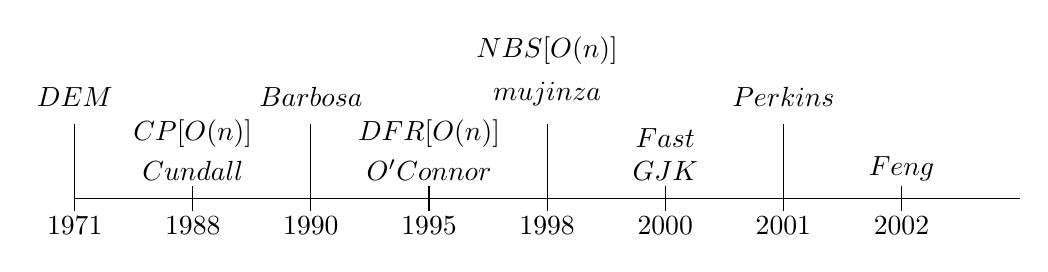
\begin{tikzpicture}[scale=1.5]
    % draw horizontal line 
    \draw (0,0) -- (8,0); 
    
    % draw vertical lines 
    \foreach \x in {1,3,5,7} 
     \draw (\x cm,3pt) -- (\x cm,-3pt); 
    \foreach \x in {0,2,4,6}
        \draw(\x cm,18pt) -- (\x cm, -3pt);
    % draw nodes 
    \draw (0,0) node[below=3pt] {$ 1971 $} node[above=30pt] {$ DEM $}; 
    \draw (1,0) node[below=3pt] {$ 1988 $} node[above=3pt] {$ Cundall $} node[above=15pt] {$ CP [O(n)] $}; 
    \draw (2,0) node[below=3pt] {$ 1990 $} node[above=30pt] {$ Barbosa $}; 
    \draw (3,0) node[below=3pt] {$ 1995 $} node[above=3pt] {$ O'Connor $} node[above = 15]{$ DFR  [O(n)] $}; 
    \draw (4,0) node[below=3pt] {$ 1998 $} node[above=30pt] {$ mujinza $}
    node[above = 45]{$ NBS  [O(n)] $}; 
    \draw (5,0) node[below=3pt] {$ 2000 $} node[above=3pt] {$ GJK $}
    node[above=15pt] {$ Fast $}; 
    \draw (6,0) node[below=3pt] {$ 2001 $} node[above=30pt] {$ Perkins $};
    \draw (7,0) node[below=3pt] {$ 2002 $} node[above=3pt] {$ Feng $};

    
    
 \end{tikzpicture}
 
 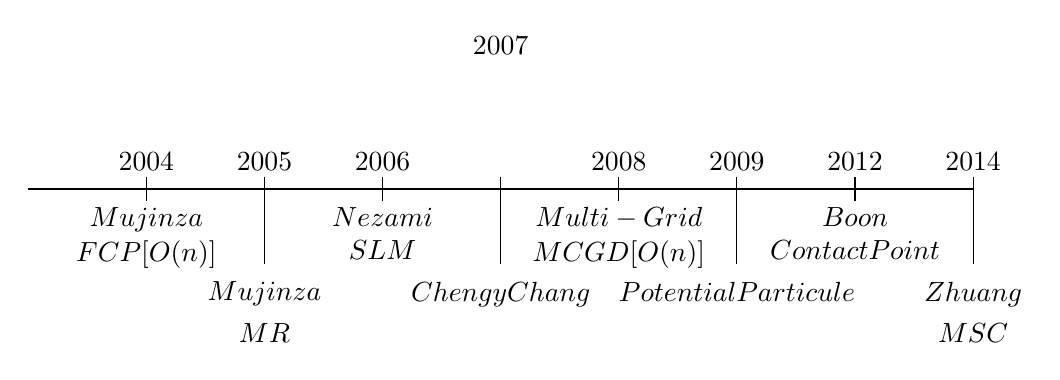
\begin{tikzpicture}[scale = 1.5]
    % draw horizontal line 
    \draw (7,0) -- (15,0); 
    
    % draw vertical lines 
    \foreach \x in {8,10,12,14} 
     \draw (\x cm,3pt) -- (\x  cm,-3pt);
    \foreach \x in {9,11,13,15}
        \draw(\x cm,3pt) -- (\x cm, -18pt);

    \draw (8,0) node[below=3pt] {$ Mujinza $} node[below=15pt] {$ FCP [O(n)] $}node[above=3pt] {$ 2004 $}; 
    \draw (9,0) node[below=30pt] {$ Mujinza $} node[below=45pt] {$ MR $} node[above=3pt] {$ 2005 $}; 
    \draw (10,0) node[below=3pt] {$ Nezami $} node[below=15pt] {$ SLM $} node[above=3pt] {$ 2006 $};
    \draw (11,0) node[below=30pt] {$ Cheng y Chang $} node[above=45pt] {$ 2007 $}; 
    \draw (12,0) node[below=3pt] {$ Multi-Grid $} node[below=15pt] {$ MCGD [O(n)] $} node[above=3pt] {$ 2008 $}; 
    \draw (13,0) node[below=30pt] {$ Potential Particule $} node[above=3pt] {$ 2009 $}; 
    \draw (14,0) node[below=3pt] {$ Boon $} node[below=15pt] {$ Contact Point $} node[above=3pt] {$ 2012 $}; 
    \draw (15,0) node[below=30pt] {$ Zhuang $} node[below=45pt] {$ MSC $} node[above=3pt] {$ 2014 $};
  
 \end{tikzpicture}

\end{frame}

\medskip
\bibliographystyle{plain}
\bibliography{/home/yerkozec/Desktop/pt/memoria/Referencia}

\end{document}
